
\documentclass{beamer}
\usecolortheme{dove}
\setbeamertemplate{navigation symbols}{}
\usepackage{amsmath,amssymb,amsfonts,amsthm, multicol, subfigure, color}
\usepackage{bm}
\usepackage{graphicx}
\usepackage{tabularx}
\usepackage{booktabs}
\usepackage{hyperref}
\usepackage{pdfpages}
\usepackage{xcolor}
\definecolor{seagreen}{RGB}{46, 139, 87}
\definecolor{mustard}{RGB}{234, 170, 0}
\def\independenT#1#2{\mathrel{\rlap{$#1#2$}\mkern2mu{#1#2}}}
\newcommand\indep{\protect\mathpalette{\protect\independenT}{\perp}}
\def\log{\text{log}}
\newcommand\logit{\text{logit}}
\newcommand\iid{\stackrel{\text{iid}}{\sim}}
\newcommand\E{\text{E}}
\newcommand\V{\text{V}}
\renewcommand\P{\text{P}}
\newcommand{\Cov}{\text{Cov}}
\newcommand{\Cor}{\text{Cor}}
\newcommand\doop{\texttt{do}}
\usepackage{stackrel}
\usepackage{tikz}
\usetikzlibrary{arrows,shapes.arrows,positioning,shapes,patterns,calc}
\newcommand\slideref[1]{\vskip .1cm \tiny \textcolor{gray}{{#1}}}
\newcommand\red[1]{\color{red}#1}
\newcommand\blue[1]{\color{blue}#1}
\newcommand\gray[1]{\color{gray}#1}
\newcommand\seagreen[1]{\color{seagreen}#1}
\newcommand\purple[1]{\color{purple}#1}
\newcommand\orange[1]{\color{orange}#1}
\newcommand\black[1]{\color{black}#1}
\newcommand\white[1]{\color{white}#1}
\newcommand\teal[1]{\color{teal}#1}
\newcommand\magenta[1]{\color{magenta}#1}
\newcommand\Fuchsia[1]{\color{Fuchsia}#1}
\newcommand\BlueGreen[1]{\color{BlueGreen}#1}
\newcommand\bblue[1]{\textcolor{blue}{\textbf{#1}}}
\newcommand\bred[1]{\textcolor{red}{\textbf{#1}}}
\newcommand\bgray[1]{\textcolor{gray}{\textbf{#1}}}
\newcommand\bgreen[1]{\textcolor{seagreen}{\textbf{#1}}}
\newcommand\bref[2]{\href{#1}{\color{blue}{#2}}}
\colorlet{lightgray}{gray!40}
\pgfdeclarelayer{bg}    % declare background layer for tikz
\pgfsetlayers{bg,main} % order layers for tikz
\newcommand\mycite[1]{\begin{scriptsize}\textcolor{darkgray}{(#1)}\end{scriptsize}}
\newcommand{\tcframe}{\frame{
%\small{
\only<1|handout:0>{\tableofcontents}
\only<2|handout:1>{\tableofcontents[currentsubsection]}}
%}
}

\newcommand{\goalsframe}{\begin{frame}{Learning goals for today}
By the end of class, you will be able to
\begin{itemize}
    \item reason about economic opportunity
    \item reason about equal opportunity
    \item connect these to a data science idea: prediction
 \end{itemize} 
  \vskip .2in
\end{frame}}

\newcommand{\credible}{\begin{frame}{Credible science}
\begin{enumerate}
\item replicability
\item reproducibility
\end{enumerate}
\end{frame}}

\usepackage[round]{natbib}
\bibliographystyle{humannat-mod}
\setbeamertemplate{enumerate items}[default]
\usepackage{mathtools}

\title{Studying Social Inequality with Data Science}
\author{Ian Lundberg}
\date{\today}

\begin{document}

\begin{frame}
\begin{tikzpicture}[x = \textwidth, y = \textheight]
\node at (0,0) {};
\node at (1,1) {};
\node[anchor = north west, align = left, font = \huge] at (0,.9) {Studying\\Social Inequality\\with Data Science};
\node[anchor = north east, align = right] (number) at (1,.9) {INFO 3370 / 5371\\Spring 2024};
\node[anchor = north, font = \Large, align = left] at (.5,.5) {\bblue{Opportunity}\\operationalized by economic mobility\\and measured by predictability};
\end{tikzpicture}
\end{frame}

\goalsframe

\begin{frame}

What does economic opportunity mean to you?

\end{frame}

\begin{frame}{Economic opportunity: Two definitions}

\begin{tabular}{rl}
\textbf{absolute mobility} & out-earning your parents \\
\textbf{relative mobility} & out-ranking your parents
\end{tabular}

\end{frame}

\begin{frame}{Absolute upward mobility: Out-earning your parents}{\bref{https://www.science.org/doi/full/10.1126/science.aal4617}{Chetty et al. 2017}}
\only<1>{
What proportion earn more than their parents at age 30?
\begin{itemize}
\item among those born in 1940
\item among those born in 1984
\end{itemize}
}
\includegraphics<2,5>[width = \textwidth]{figures/chetty2017_fig1b}
\includegraphics<3>[width = .8\textwidth]{figures/chetty2017_fig2b}
\includegraphics<4>[width = .8\textwidth]{figures/chetty2017_fig2c}
\end{frame}

\begin{frame}{Economic opportunity: Two definitions}

\begin{tabular}{rll}
\textbf{absolute mobility} & out-earning your parents & has fallen \\
\textbf{relative mobility} & out-ranking your parents
\end{tabular}

\end{frame}

\begin{frame}
\begin{tikzpicture}[x = \textwidth, y = \textheight]
\node at (0,0) {};
\node at (1,1) {};
\node<1-3>[anchor = north west, align = left] (title) at (.6,.8) {\textbf{absolute upward}\\\textbf{mobility}};
\node<1-3>[anchor = north west, align = left] at (title.south west) {landing higher than\\your parents in\\dollars};
\node<1,3>[anchor = west] at (0,.5) {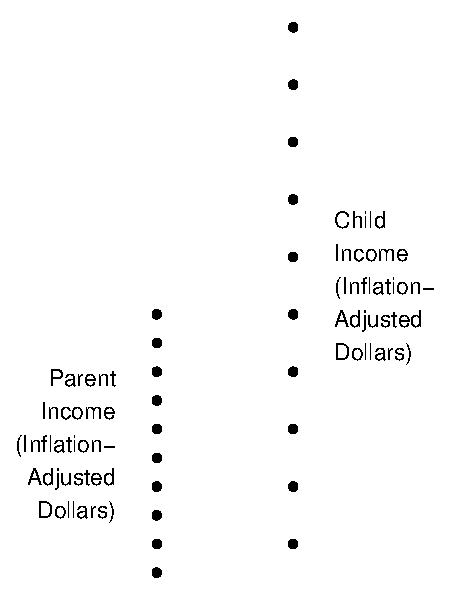
\includegraphics[height = .8\textheight]{abs_mobility_1}};
\node<2>[anchor = west] at (0,.5) {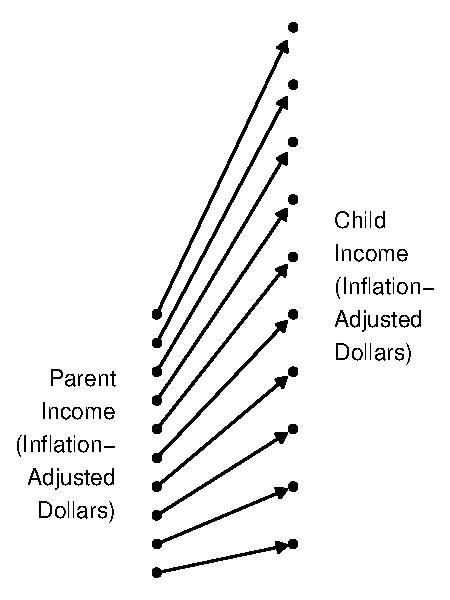
\includegraphics[height = .8\textheight]{abs_mobility_2}};
\node<4>[anchor = west] at (0,.5) {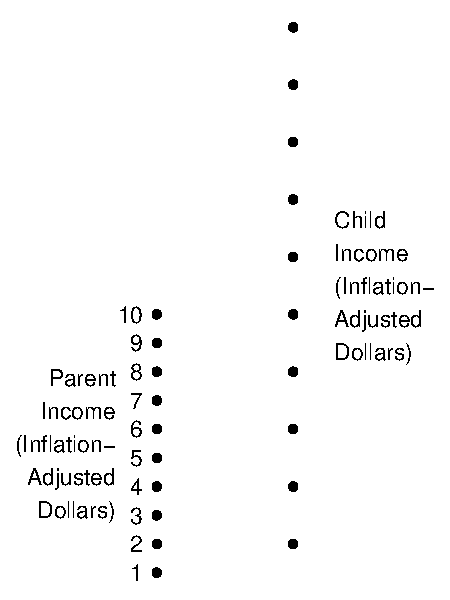
\includegraphics[height = .8\textheight]{rank_parents}};
\node<5>[anchor = west] at (0,.5) {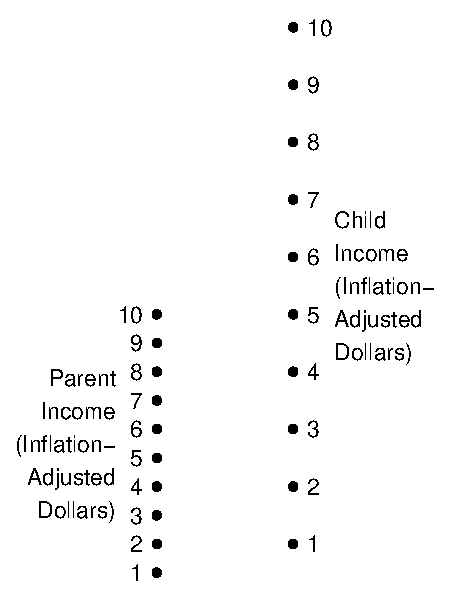
\includegraphics[height = .8\textheight]{rank_children}};
\node<6-7>[anchor = west] at (0,.5) {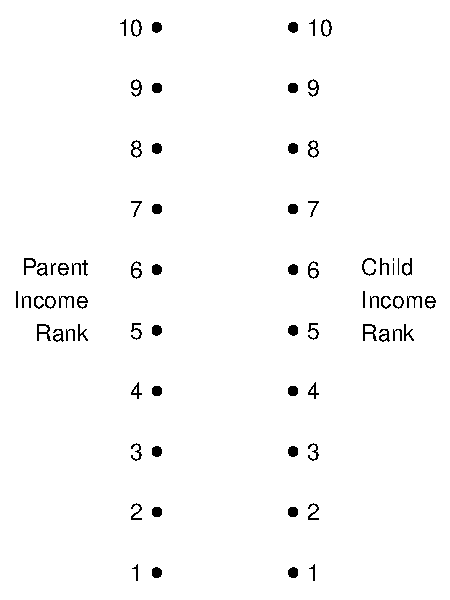
\includegraphics[height = .8\textheight]{ranks_base}};
\node<7->[anchor = north west, align = left] (title) at (.6,.8) {\textbf{relative upward}\\\textbf{mobility}};
\node<7->[anchor = north west, align = left] at (title.south west) {landing higher than\\your parents in\\ranks};
\node<8>[anchor = west] at (0,.5) {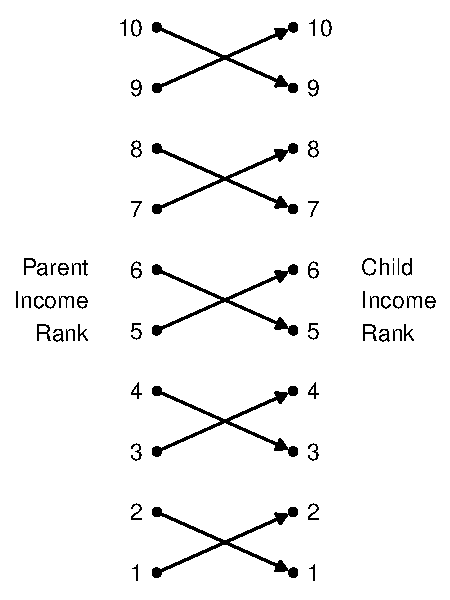
\includegraphics[height = .8\textheight]{ranks_50pct}};
\node<8>[anchor = north west, align = left] at (.6,.4) {\textbf{example}\\half move up\\half move down};
\node<9->[anchor = north west, align = left] at (.6,.4) {\textbf{example}\\90\% move up};
\node<9>[anchor = west] at (0,.5) {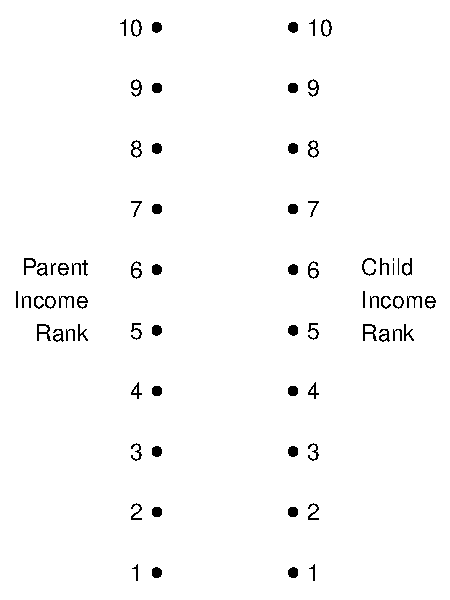
\includegraphics[height = .8\textheight]{ranks_base}};
\node<10>[anchor = west] at (0,.5) {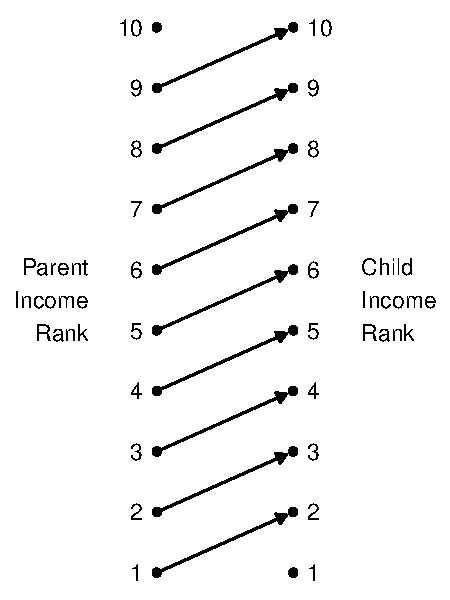
\includegraphics[height = .8\textheight]{ranks_90pct_1}};
\node<11>[anchor = west] at (0,.5) {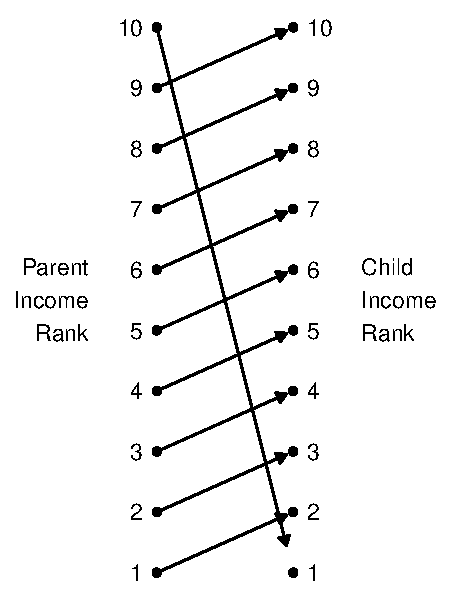
\includegraphics[height = .8\textheight]{ranks_90pct_2}};
\end{tikzpicture}
\end{frame}

\begin{frame}{Relative upward mobility: Reaching the top}{\bref{https://eml.berkeley.edu/~saez/chettyetalAERPP2014.pdf}{Chetty et al. 2014}}
\begin{tikzpicture}[x = \textwidth, y = \textheight]
\node<2>[anchor = west] at (0,.5) {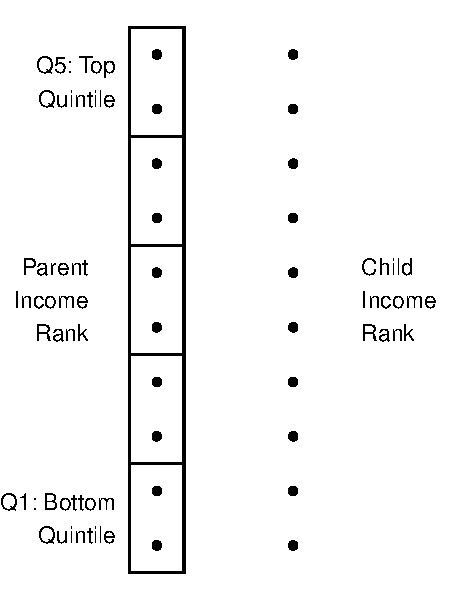
\includegraphics[height = .7\textheight]{ranks_quintiles_1}};
\node<3>[anchor = west] at (0,.5) {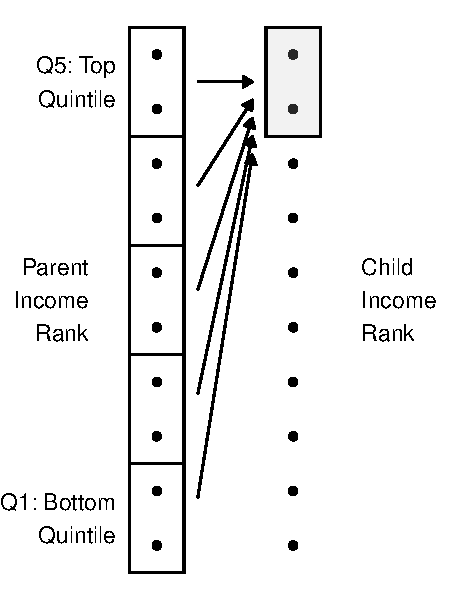
\includegraphics[height = .7\textheight]{ranks_quintiles_2}};
\node<4>[anchor = west] at (0,.5) {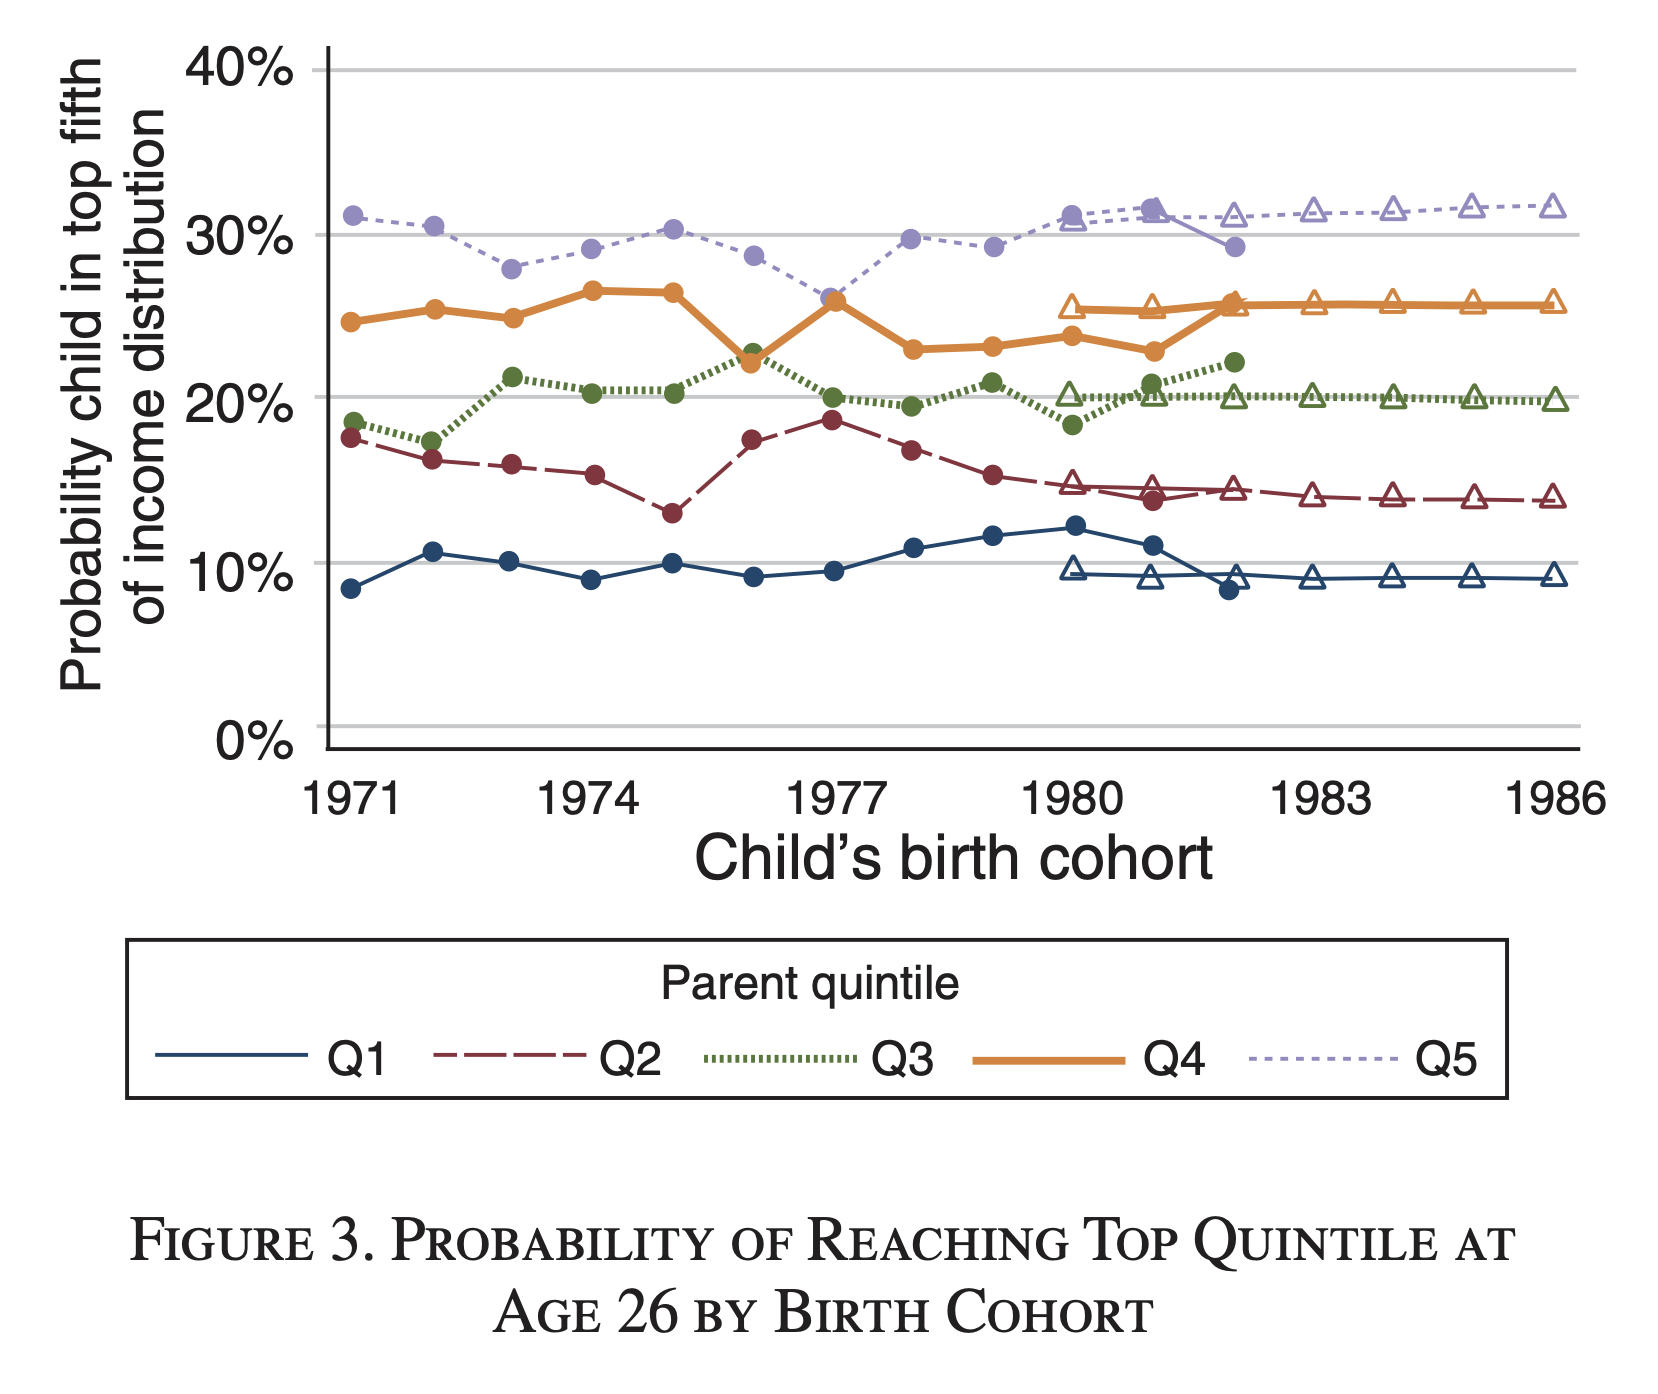
\includegraphics[height = .7\textheight]{figures/chetty_fig3}};
\end{tikzpicture}
\end{frame}

\begin{frame}{Economic opportunity: Two definitions}

\begin{tabular}{rll}
\textbf{absolute mobility} & out-earning your parents & has fallen \\
\textbf{relative mobility} & out-ranking your parents & roughly constant
\end{tabular}

\end{frame}

\begin{frame}

What does \textbf{equal} opportunity mean to you?

\end{frame}

\begin{frame}

Now, the premise that we’re all created equal is the opening line in the American story. And while we don’t promise equal outcomes, we’ve strived to deliver equal opportunity -- the idea that success doesn’t depend on being born into wealth or privilege, it depends on effort and merit. \vskip .2in

--- Barack Obama, \bref{https://www.washingtonpost.com/politics/running-transcript-president-obamas-december-4-remarks-on-the-economy/2013/12/04/7cec31ba-5cff-11e3-be07-006c776266ed_story.html}{Remarks on the Economy}, Dec 2013. \bref{https://youtu.be/bXjksBH9QZE?t=266}{[Video]} \vskip .3in \pause

\begin{center}
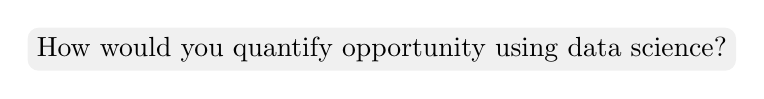
\begin{tikzpicture}
\node[fill = lightgray, rounded corners, fill opacity = .3, text opacity = 1] at (0,0) {How would you quantify opportunity using data science?};
\end{tikzpicture}
\end{center}

\end{frame}



\begin{frame}
\begin{tikzpicture}[x = \textwidth, y = \textheight]
\node[anchor = west] (eq) at (.5,.5) {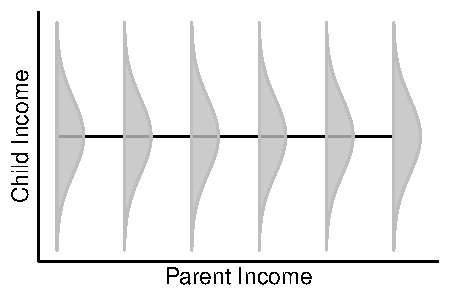
\includegraphics[width = .4\textwidth]{equal}};
\node[anchor = south west] at (eq.north west) {Equal Opportunity}; \pause
\node[anchor = west] (un) at (0,.5) {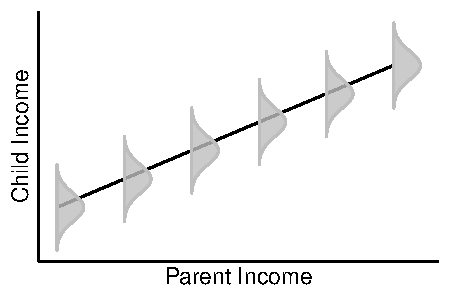
\includegraphics[width = .4\textwidth]{unequal}};
\node[anchor = south west] at (un.north west) {Unequal Opportunity}; \pause
\node[anchor = north west, align = left] at (0,.3) {Child outcomes are \textbf{predictable}\\given family background};
\node[anchor = north west, align = left] at (.5,.3) {Child outcomes are \textbf{unpredictable}\\given family background};
\end{tikzpicture}

\end{frame}

\begin{frame}
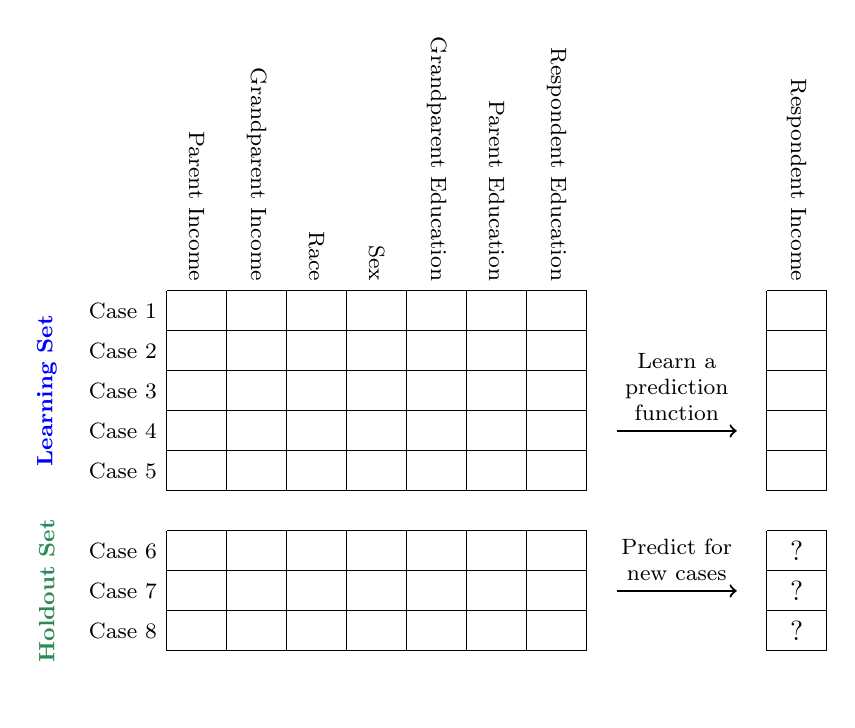
\begin{tikzpicture}[x = 3in, y = 2in]
\node[anchor = east, rotate = 270, font = \footnotesize] at (.15,1) {Parent Income};
\node[anchor = east, rotate = 270, font = \footnotesize] at (.25,1) {Grandparent Income};
\node[anchor = east, rotate = 270, font = \footnotesize] at (.35,1) {Race};
\node[anchor = east, rotate = 270, font = \footnotesize] at (.45,1) {Sex};
\node[anchor = east, rotate = 270, font = \footnotesize] at (.55,1) {Grandparent Education};
\node[anchor = east, rotate = 270, font = \footnotesize] at (.65,1) {Parent Education};
\node[anchor = east, rotate = 270, font = \footnotesize] at (.75,1) {Respondent Education};
\node[anchor = east, font = \footnotesize] at (.1,.95) {Case 1};
\node[anchor = east, font = \footnotesize] at (.1,.85) {Case 2};
\node[anchor = east, font = \footnotesize] at (.1,.75) {Case 3};
\node[anchor = east, font = \footnotesize] at (.1,.65) {Case 4};
\node[anchor = east, font = \footnotesize] at (.1,.55) {Case 5};
\draw[step=.1,black,thin] (0.1,.5) grid (.8,1); 
\node at (.5,1) {};
\pause
\node[anchor = east, rotate = 270, font = \footnotesize] at (1.15,1) {Respondent Income};
\draw[step=.1,black,thin] (1.1,.5) grid (1.2,1);
\draw[thin] (1.2,.5) -- (1.2,1);
\pause
\draw[->, thick] (.85,.65) -- node[midway, above, font = \footnotesize, align = center] {Learn a\\prediction\\function} (1.05,.65);
\pause
% Holdout set
\draw[step=.1,black,thin] (0.1,.1) grid (.8,.4);
\draw[step=.1,black,thin] (1.1,.1) grid (1.2,.4);
\draw[thin] (1.2,.1) -- (1.2,.4);
\node at (1.15,.35) {?};
\node at (1.15,.25) {?};
\node at (1.15,.15) {?};
\node[anchor = east, font = \footnotesize] at (.1,.35) {Case 6};
\node[anchor = east, font = \footnotesize] at (.1,.25) {Case 7};
\node[anchor = east, font = \footnotesize] at (.1,.15) {Case 8};
\pause
\draw[->, thick] (.85,.25) -- node[midway, above, font = \footnotesize, align = center] {Predict for\\new cases} (1.05,.25);
\pause
% Label the two
\node[rotate = 90, font = {\footnotesize\bf}, blue] at (-.1,.75) {{Learning} Set};
\node[rotate = 90, font = {\footnotesize\bf}, seagreen] at (-.1,.25) {{Holdout} Set};
\node at (-.05,0) {};
\end{tikzpicture}
\end{frame}

\begin{frame}{The challenge}
How well can you predict respondent incomes? \vskip .2in
Get started \bref{https://info3370.github.io/lessonplans/7b/}{here}
\end{frame}

\goalsframe

\end{document}

